\chapter{پیاده‌سازی}

در بخش قبلی معماري کلی سامانه و ماژول‌هاي موردنیاز براي پیاده سازي سامانه پایش شبکه را بیان و به صورت اجمالی معرفی کردیم. در این فصل به چگونگی قرار گرفتن و ارتباط بخش‌هاي مختلف می‌پردازیم و پیاده سازي سیستم را توضیح خواهیم داد.


ماژول‌های تعریف شده در فصل قبل برای سامانه پایش شبکه‌های کامپیوتری را می‌توان در چهار دسته کلی قرار داد: 

\begin{itemize}
    \item هسته \lr{SNMP}
    \item فرانت‌اند 
    \item بک‌اند
    \item ذخیره‌سازی اطلاعات


\end{itemize}

در ادامه برای هر دسته توضیحاتی ارائه خواهد شد. این توضیحات شامل ماژول‌های دربرگیرنده آن، بررسی راه‌های ممکن برای پیاده‌سازی هر ماژول و درنهایت نحوه پیاده‌سازی آن ماژول خواهد بود. 


\section{هسته \lr{SNMP}}

این دسته فقط شامل ماژول هسته \lr{SNMP} از \cref{fig.11} است. برای این ماژول هدف، توسعه ابزاری است که بتوان از طریق آن انواع پیام‌های \lr{SNMP} را ارسال و دریافت کرد. بدین منظور با تعریف دو کلاس \lr{Trap} و \lr{Session} این ماژول را پیاده‌سازی می‌کنیم. توجه شود که کتابخانه \lr{net-snmp} به زبان \lr{C} است ولی این ماژول جهت توسعه بهینه در زبان \lr{C++} توسعه داده شد. در نهایت ابزاری برای این ماژول تولید شد که قابلیت دریافت پیام‌های \lr{Trap} از طریق کلاس \lr{Trap} و همچنین  ارسال و دریافت \lr{get} و \lr{walk} از طریق کلاس \lr{ Session } را دارد.

\newpage

\section{فرانت‌اند}

این دسته فقط شامل ماژول رابط کاربری تحت وب از \cref{fig.11} است. این قسمت برای توسعه بهینه همانطور که در فصل قبل گفته شد با فریمورک ری‌اکت توسعه داده شد. در این قسمت قدم به قدم رابط کاربری توسعه داده شده به همراه کارایی آن مورد بررسی قرار می‌دهیم.


در \cref{fig.12} و \cref{fig.13} منو‌های سامانه نشان داده می‌شود که شرح مختصری از آن‌ها در ادامه آورده شده است:


\begin{figure}[!h]
    \centering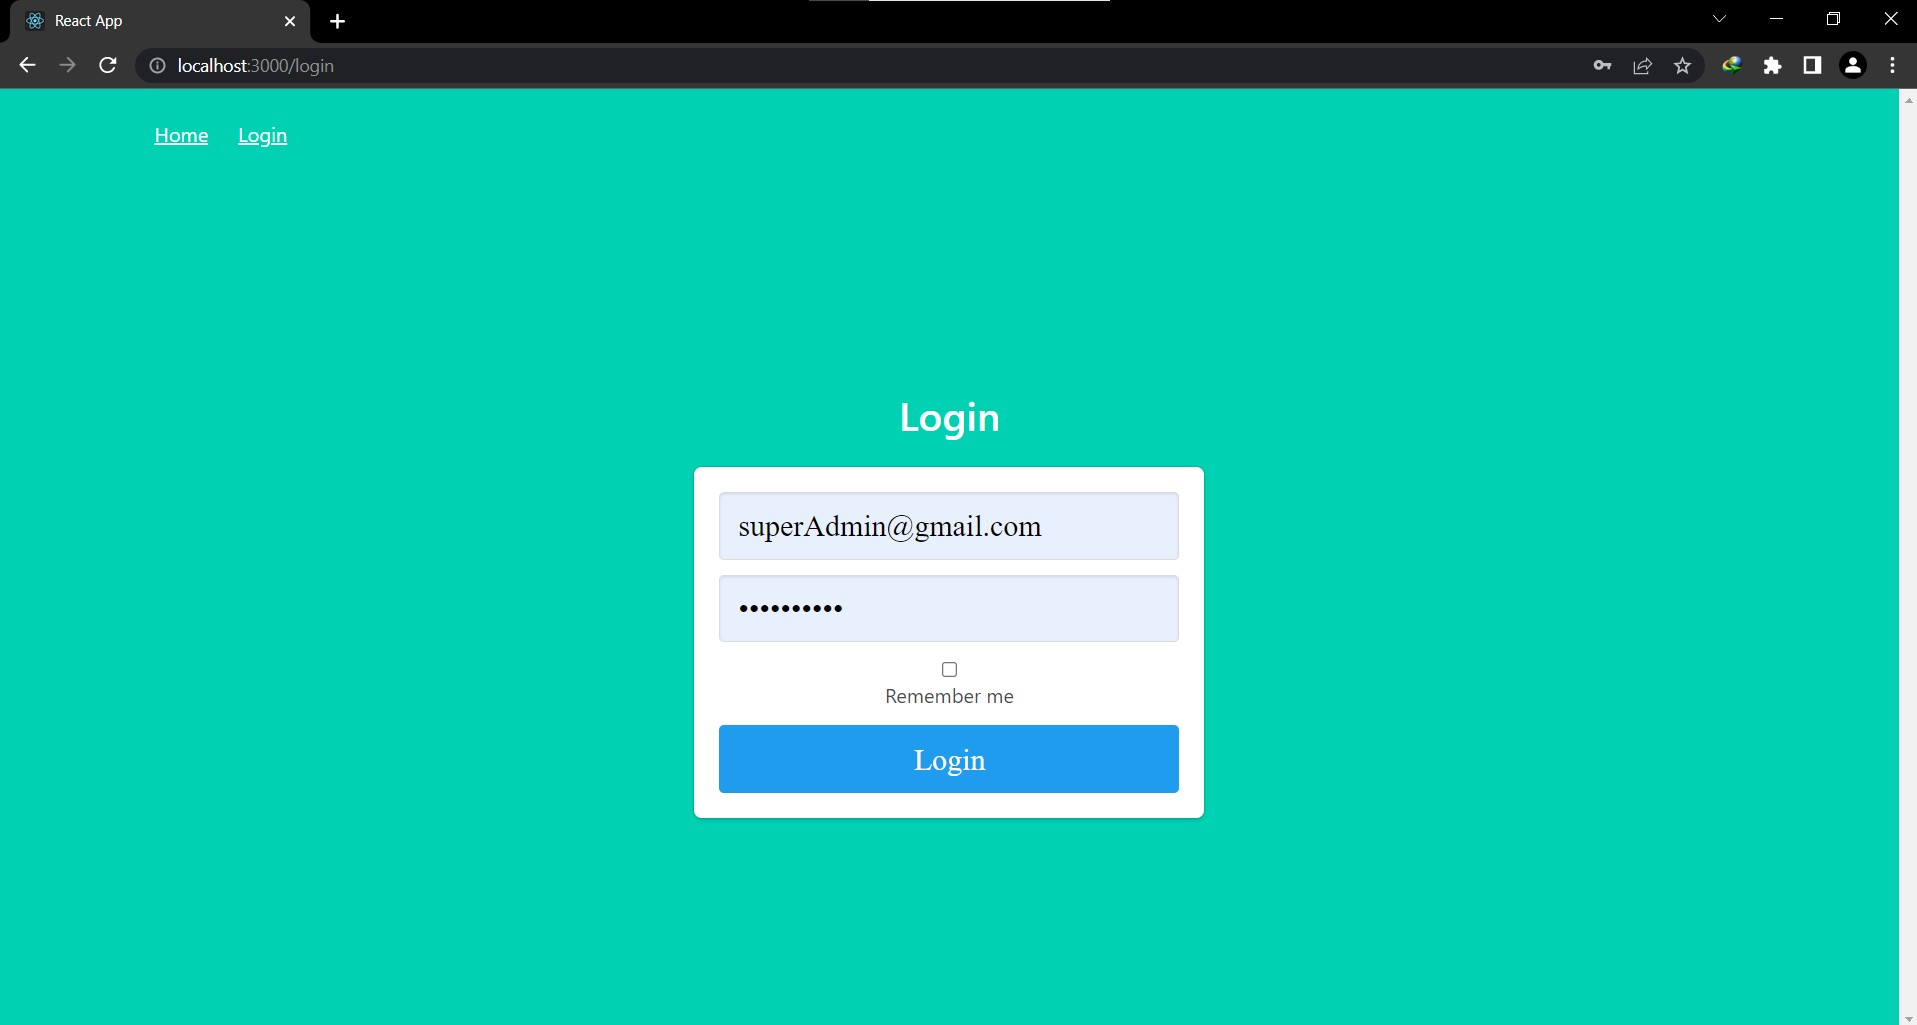
\includegraphics[scale=.38]{./nav-logout}
    \caption{منوی سیستم هنگام لاگین}\label{fig.12}
\end{figure}

\begin{figure}[!h]
    \centering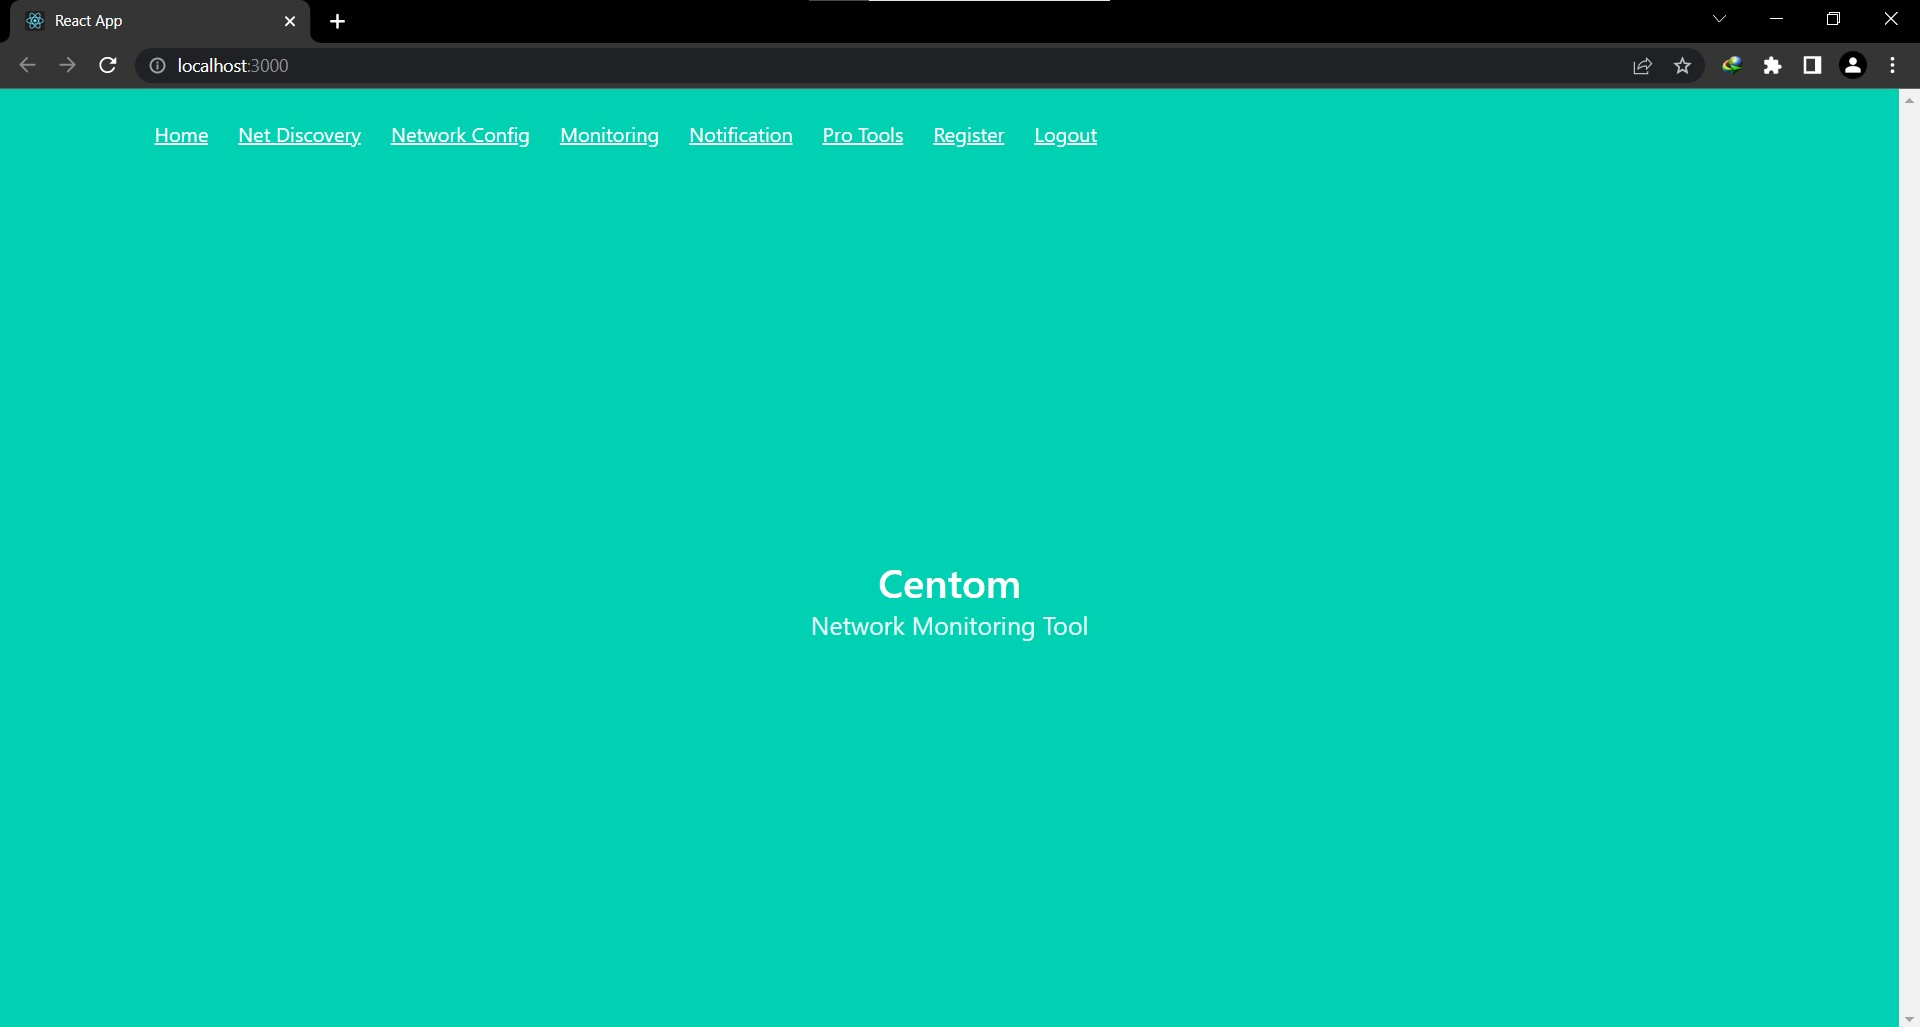
\includegraphics[scale=.38]{./nav-login}
    \caption{منوی سیستم بعد از لاگین ادمین ارشد}\label{fig.13}
\end{figure}
        
زمانی که کاربری لاگین نکرده است(\cref{fig.12})، تنها دو صفحه خانه و لاگین قابل دسترسی خواهد بود. این بدان علت است که در این سامانه ثبت نام کاربر فقط توسط ادمین ارشد صورت می‌گیرد. در \cref{fig.13} منوها پس از لاگین ادمین ارشد نمایش داده شده‌اند. تاکیر بر روی ادمین ارشد بدین علت است که در این سامانه سه سطح دسترسی ادمین ارشد، ادمین معمولی و کاربر عادی وجود دارد. ادمین ارشد به همه امکانات، ادمین معمولی به ثبت نام کاربر جدید، تنظیمات و اسکن شبکه دسترسی ندارد. کاربر عادی نیز فقط به اسکن سریع یک دستگاه دسترسی خواهد داشت. البته این سامانه فقط یک ادمین ارشد خواهد داشت!

\newpage

تعریف کاربر جدید فقط توسط ادمین ارشد تحت رجیستر در \cref{fig.14} ممکن خواهد بود. برای ثبت نام یک کاربر، ادمین ارشد باید یک ایمیل، رمز عبور وارد نماید. سپس باید بین دو نقش ادمین معمولی ویا کاربر معمولی انتخاب نماید. در نهایت ایمیل و رمز عبور را در اختیار شخص متقاضی قرار می‌دهد.


\begin{figure}[!h]
    \centering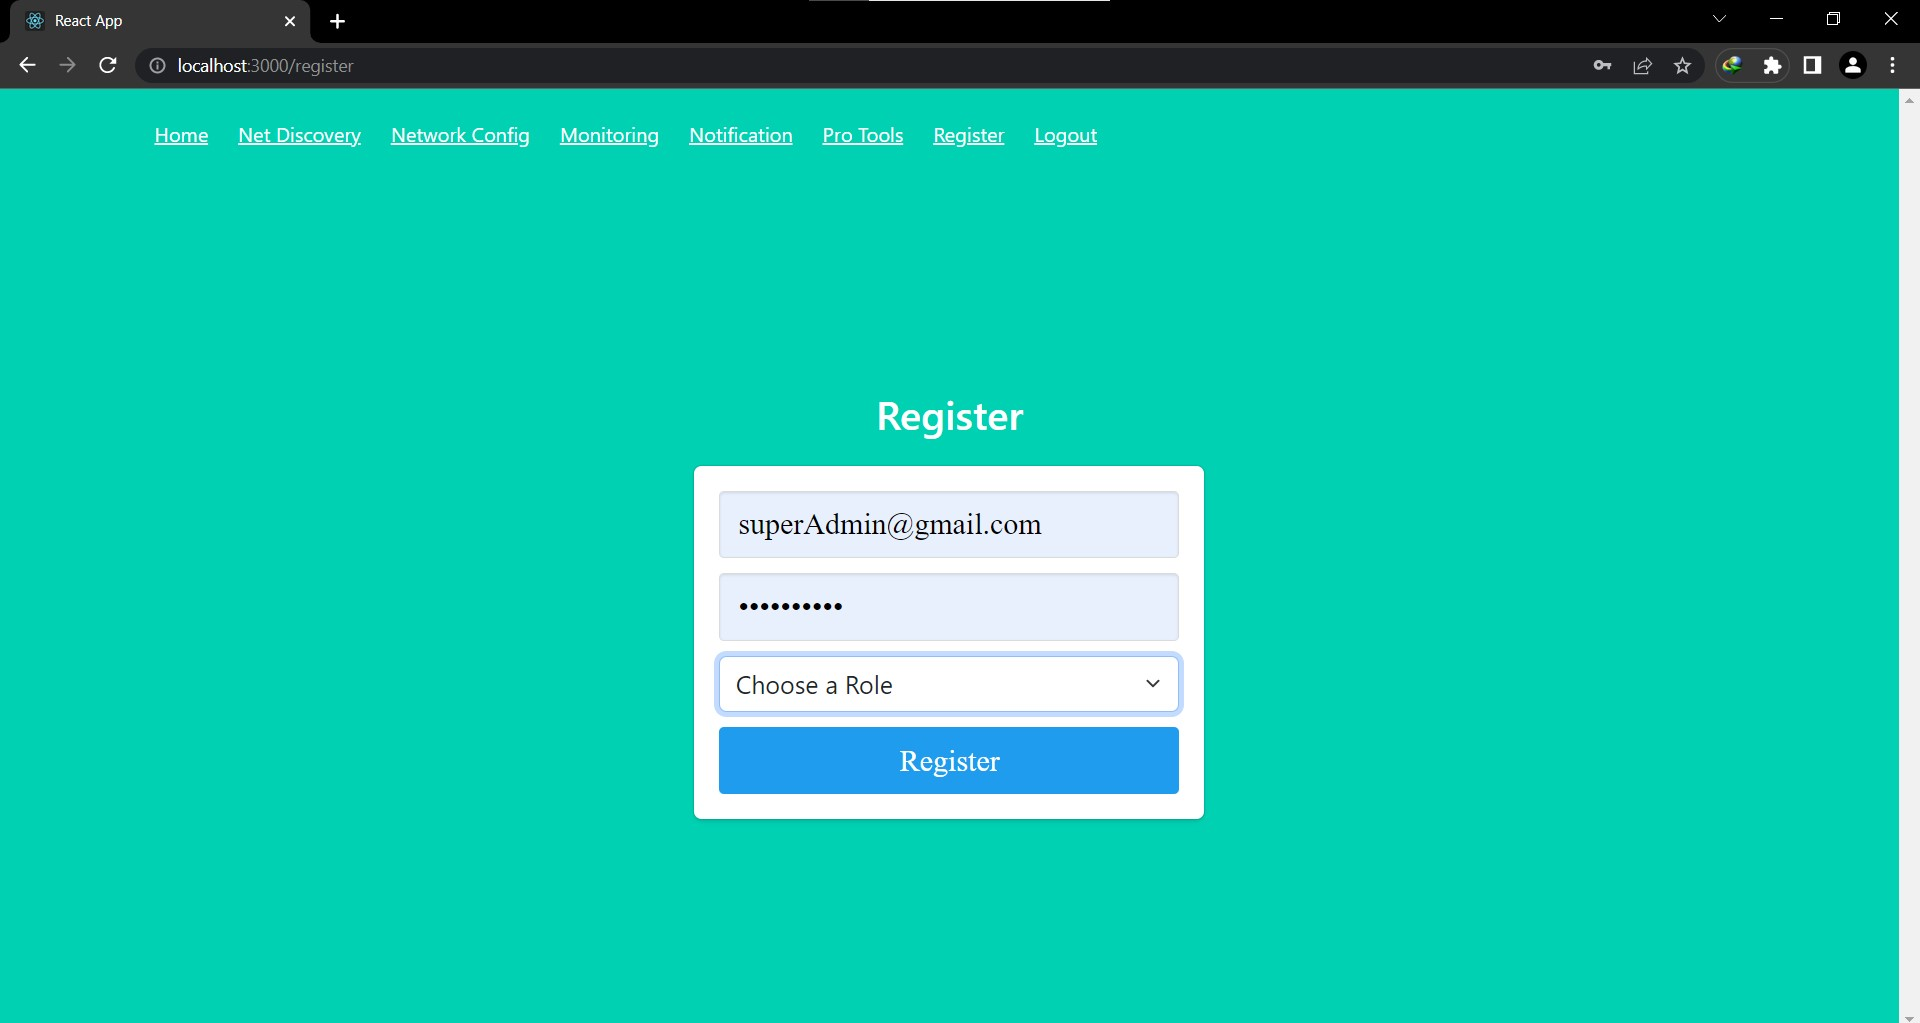
\includegraphics[scale=.38]{./register}
    \caption{صفحه رجیستر در اختیار ادمین ارشد}\label{fig.14}
\end{figure}


مهم‌ترین قسمت این سامانه، کشف شبکه است که اولین منو بعد از منوی خانه قرار دارد. رابط کاربری این قسمت قبل و بعد از تست در \cref{fig.15} و \cref{fig.16} نشان داده شده‌ است. 


\begin{figure}[!h]
    \centering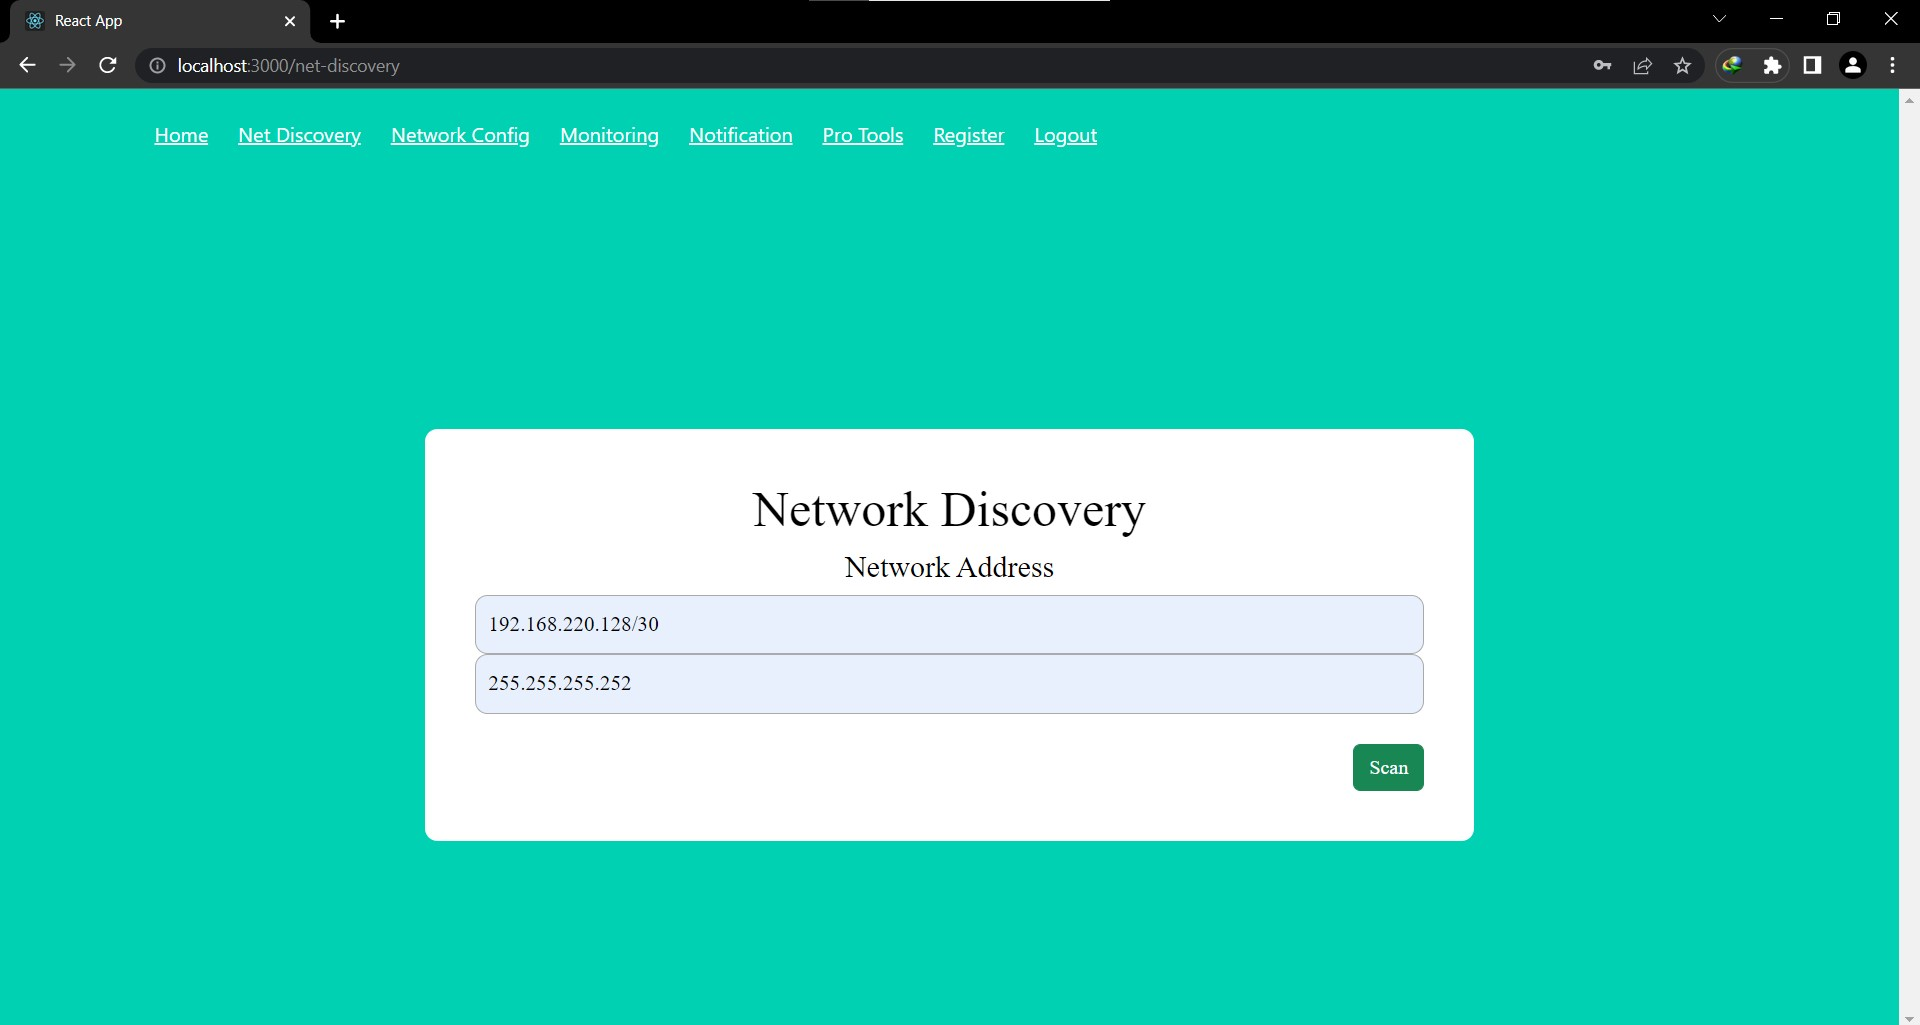
\includegraphics[scale=.38]{./net-dis-before}
    \caption{صفحه کشف شبکه قبل از اسکن}\label{fig.15}
\end{figure}


\begin{figure}[!h]
    \centering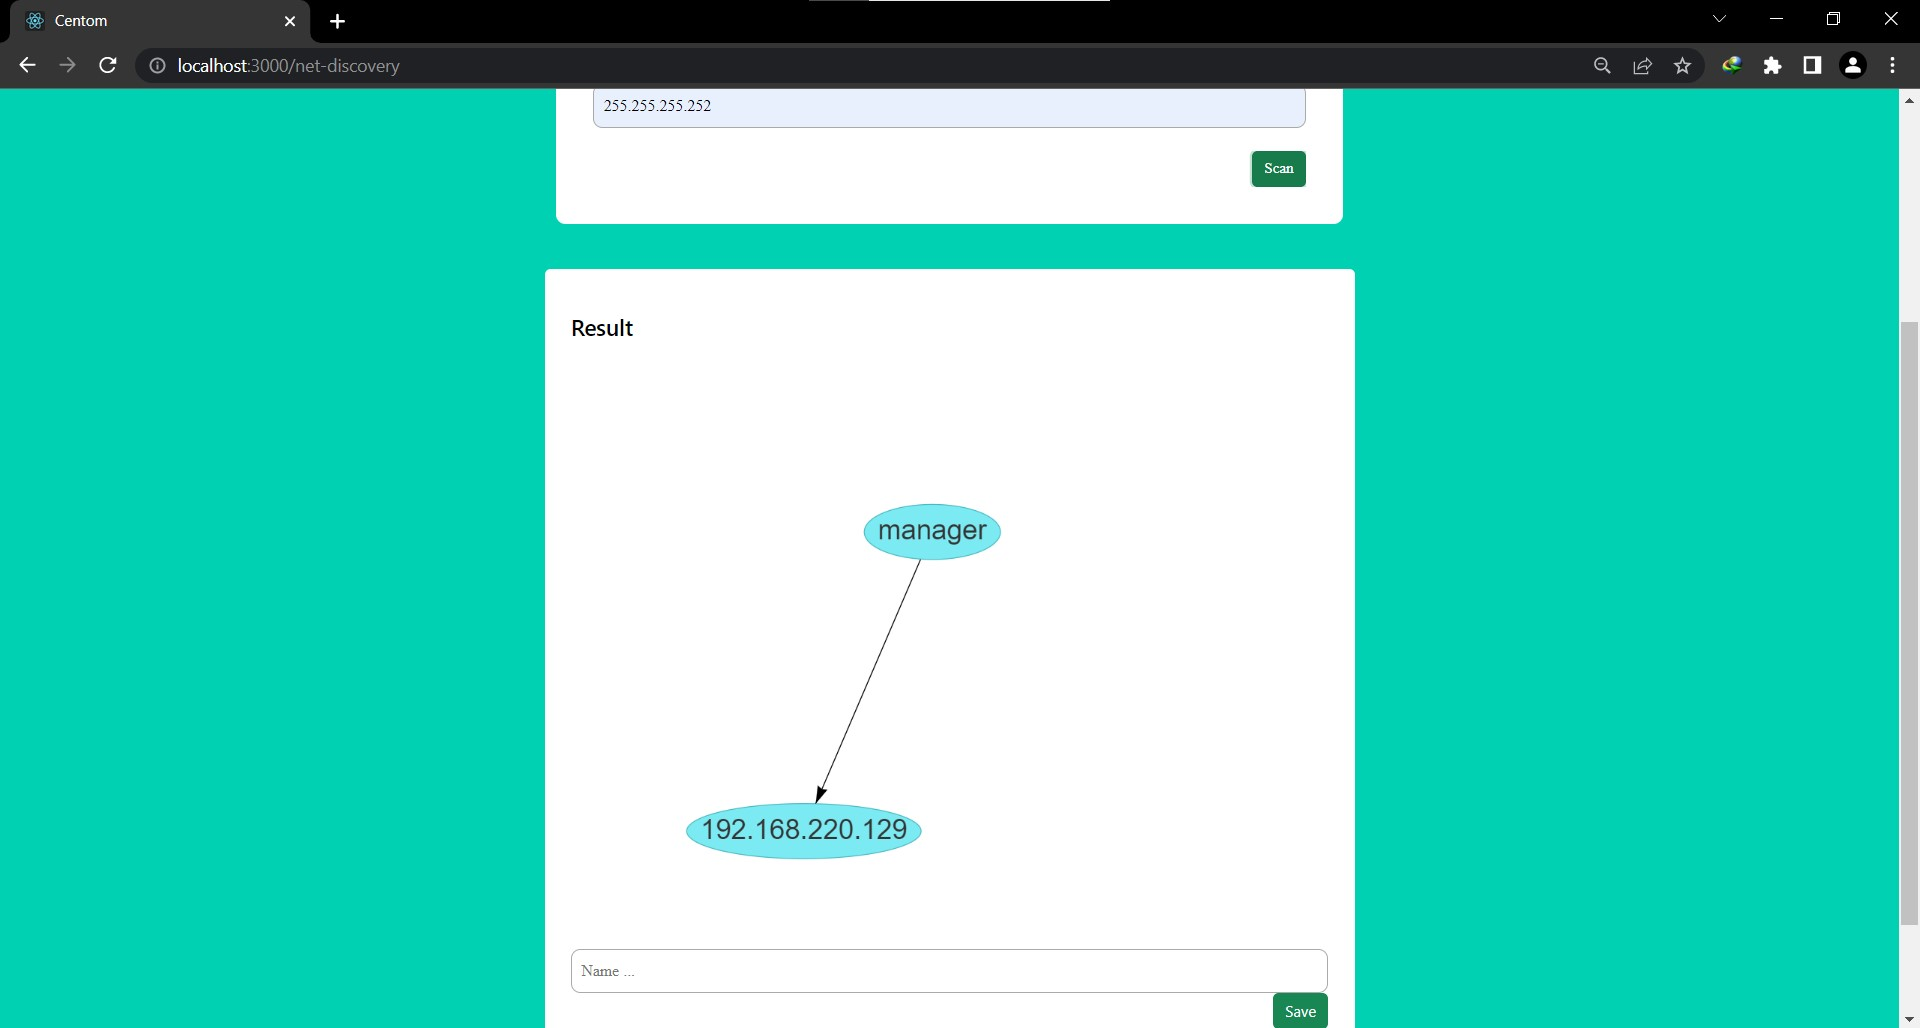
\includegraphics[scale=.38]{./net-dis-after}
    \caption{خروجی اسکن شبکه در قالب یک گراف}\label{fig.16}
\end{figure}


در کشف شبکه ابتدا یک آدرس شبکه به همراه \lr{Subnet Mask} از ادمین ارشد گرفته می‌شود. سپس بعد از اتمام اسکن شبکه، خروجی در قالب یک گراف نمایش داده می‌شود. درنهایت ادمین ارشد می‌تواند در صورت نیاز شبکه را با اسمی دلخواه در سامانه ذخیره کند.


بعد از ذخیره‌ سازی شبکه در قسمت قبل، ادمین ارشد می‌تواند ابتدا اطلاعات و تنظیمات شبکه را وارد نماید و بعد از آن اقدام به پایش شبکه کند. بدین ترتیب بعد از منوی کشف شبکه، منوی ذخیره تنظیمات شبکه در \cref{fig.17} وجود دارد. ابتدا با انتخاب اسم شبکه و نوع دستگاه‌های مورد نظر سامانه لیستی از آدرس‌ها را نشان می‌دهد. که با انتخاب یک آدرس مشخصات آن توسط کاربر وارد می‌شود. همچنین می‌تواند پارامترهای مورد نظر برای پایش دستگاه را به صورت لیست اضافه کند.



\begin{figure}[!h]
    \centering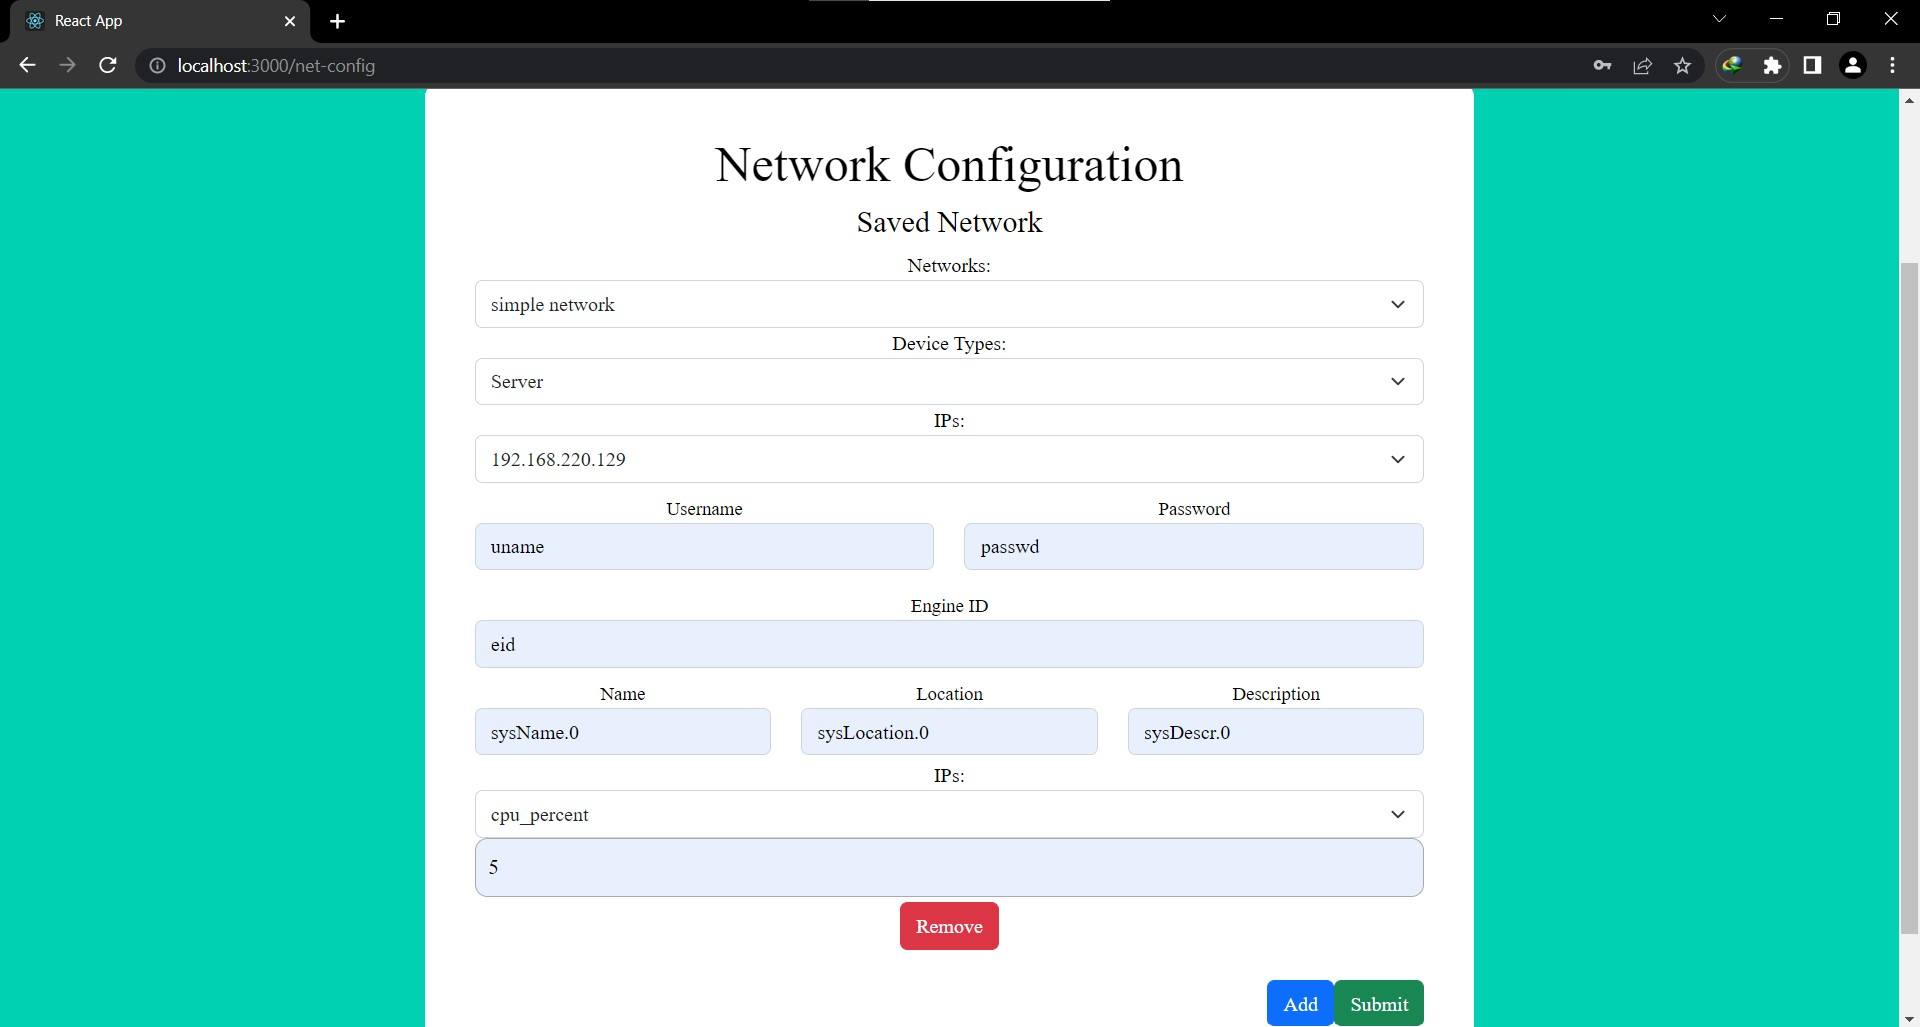
\includegraphics[scale=.38]{./net-config}
    \caption{صفحه ذخیره تنظیمات شبکه}\label{fig.17}
\end{figure}





% مانیتورینگ ///////////////////////////////////////////////////////////////////////////////////////////////////////
% نوتیفیکیشن //////////////////////////////////////////////////////////////////////////////////////////////////////


در نهایت منوی ابزارهای پیشرفته قرار دارد، که در حال حاضر تنها اسکن سریع آن در \cref{fig.120} موجود است. سامانه در این قسمت می‌تواند با دریافت یک آدرس و یک شناسه شی، پیام‌های \lr{get} و \lr{walk} را ارسال و نتیجه را به ترتیب مشاهده کند. 

\begin{figure}[!h]
    \centering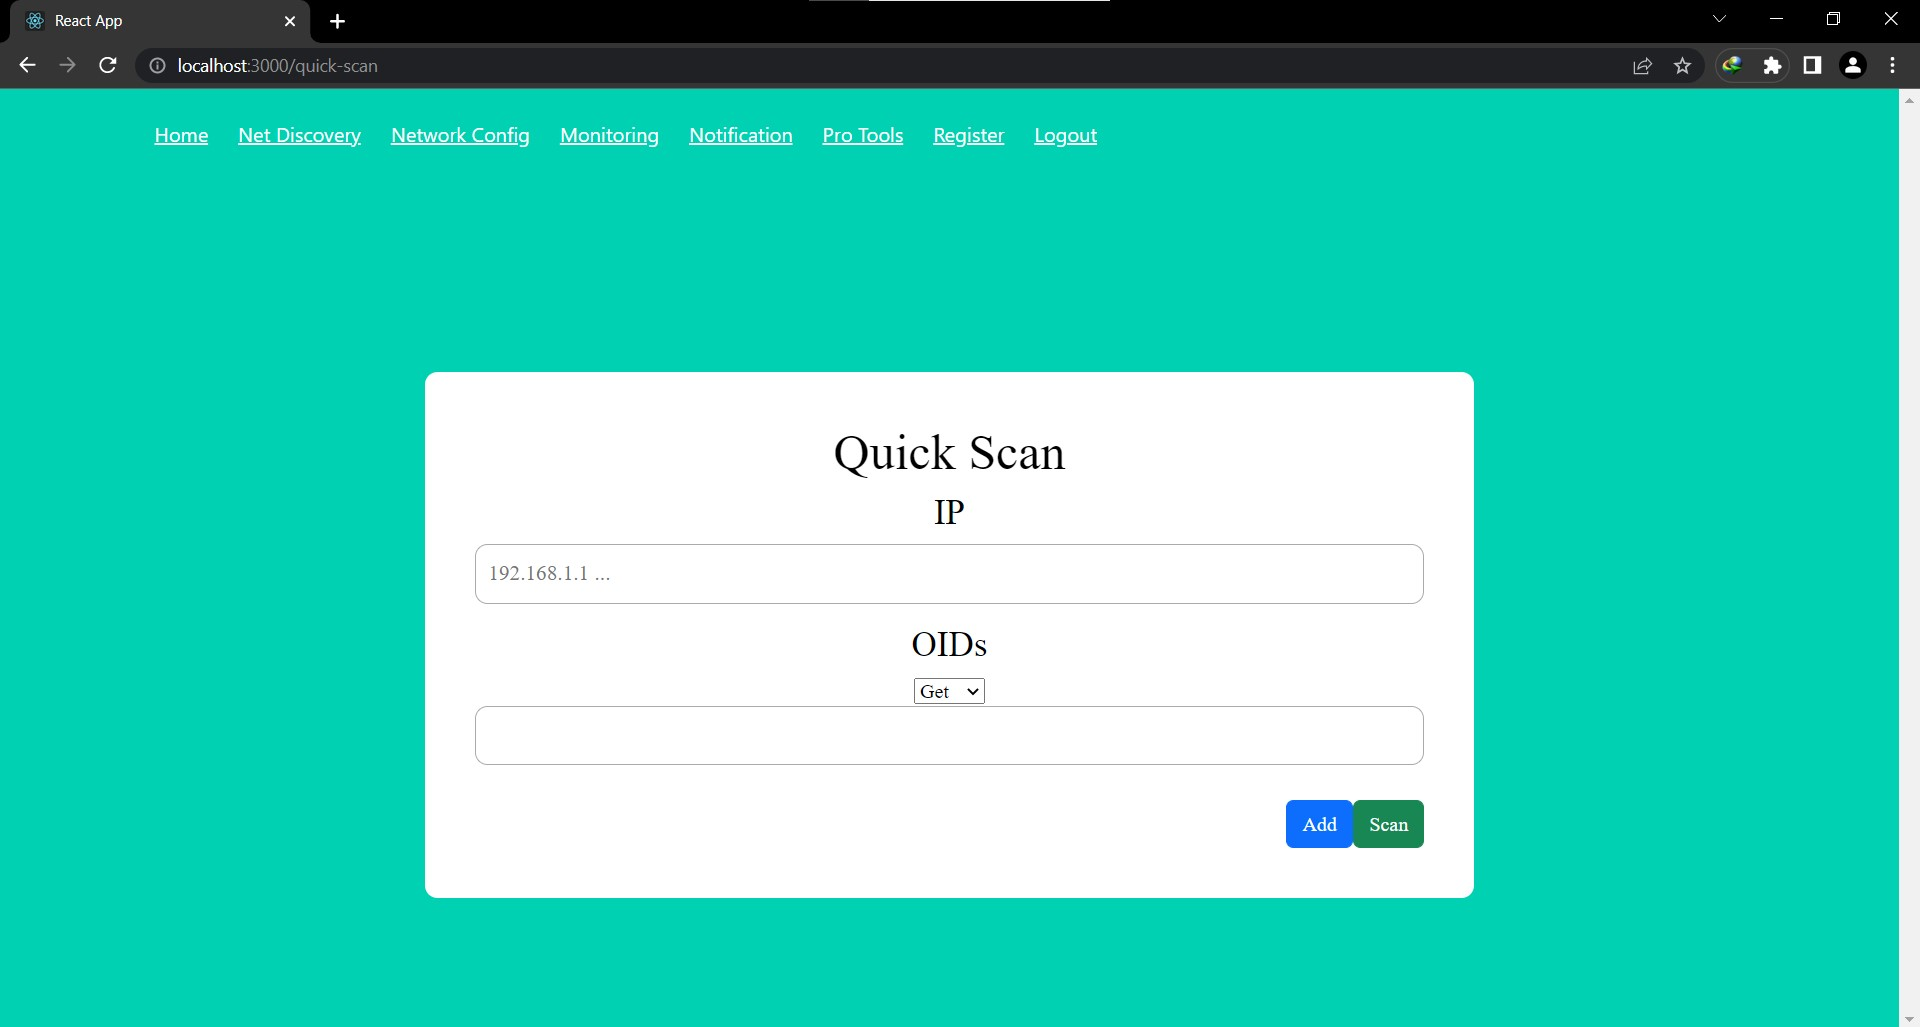
\includegraphics[scale=.38]{./pro-tools}
    \caption{صفحه ابزارهای پیشرفته}\label{fig.120}
\end{figure}



\newpage

\section{ذخیره‌سازی اطلاعات}

این دسته فقط شامل ماژول ذخیره سازی اطلاعات شبکه از شکل \cref{fig.11} است. در این سامانه به طور کلی سه نوع داده کاربران، اطلاعات شبکه و اطلاعات دریافتی از عناصر تحت مدیریت شبکه وجود دارد. 



\subsection{ذخیره‌سازی اطلاعات شبکه و کاربران}

برای ذخیره سازی اطلاعات کاربران و اطلاعات شبکه از پایگاه داده \lr{SQLite} با تعریف جداول شکل \cref{fig.121} استفاده می‌کنیم.

\begin{figure}[!h]
    \centering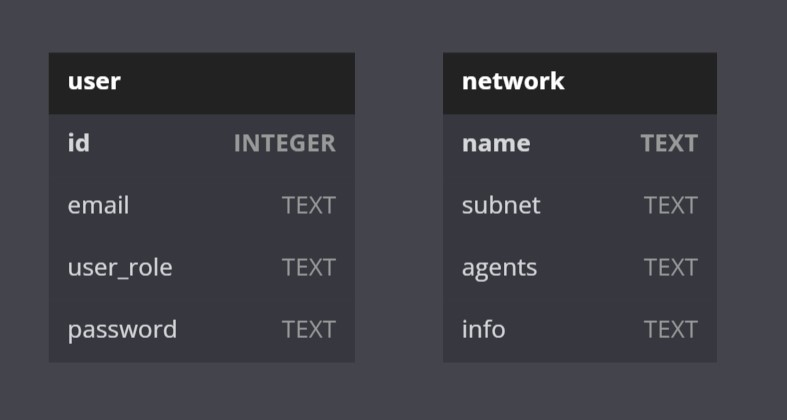
\includegraphics[scale=.60]{./db}
    \caption{تصویر جداول تعریف شده در پایگاه داده \lr{SQLite}}\label{fig.121}
\end{figure}


فیلدهایی که نیاز است توضیحی درباره آن‌ها داده شود به صورت زیر است:

\begin{itemize}
    \item \lr{user-role}: نقش هر کاربر جهت دسترسی ‌های متنوع به سامانه را می‌دهد. به عنوان مثال ادمین ارشد به همه امکانات، ادمین معمولی به همه امکانات به جز ثبت نام کاربر جدید، تنظیمات و اسکن شبکه دسترسی دارند. و در نهایت کاربر عادی فقط به اسکن سریع یک دستگاه دسترسی خواهد داشت.
    \item \lr{name}: این فیلد فقط برای شناسایی متمایز شبکه‌ها کاربرد دارد. بدین صورت که با دریافت یک اسم از کاربر به هنگام ذخیره، تنها زمان بازیابی اطلاعات شبکه در سامانه کاربرد دارد.
    \item \lr{agents}: این فیلد شامل لیستی از دستگاه‌های شبکه است که عامل \lr{SNMP} بر روی آن‌ها فعال است.
    \item \lr{info}: این فیلد شامل شی‌ای از \lr{JSON} شامل گره‌ها، یال‌ها و نوع دستگاه‌های تحت مدیریت است.

\end{itemize}


برای اتصال به پایگاه داده \lr{SQLite} نیز از \lr{SQLAlchemy} که یک ابزار نگاشت رابطه به شی است، استفاده شد که مزایای بسیاری دارد.



\subsection{ذخیره‌سازی اطلاعات دریافتی از شبکه}

این اطلاعات در درجه اول شامل پارامتر‌های مختلف جهت پایش دستگاه‌ها به همراه نرخ نمونه برداری آن‌ها است. در درجه بعد شامل اطلاعات دریافتی از دستگاه‌های تحت مدیریت مربوط به پارامترهای مختلف خواهد بود. به علت تعداد بالای بازیابی این گونه اطلاعات از ردیس استفاده کردیم. برای اتصال به ردیس نیز از ماژول \lr{redis} در پایتون استفاده شد.

\newpage

\section{بک‌اند}

این دسته شامل ماژول‌های پردازش اطلاعات شبکه، هشدار، کشف شبکه و جمع‌آوری اطلاعات (مانیتورینگ) از شکل \cref{fig.11} است.

\subsection{ماژول کشف شبکه}

در این ماژول با توجه به نیازمندی‌های گفته شده در فصل تحلیل و طراحی، باید با دریافت یک آدرس شبکه  سامانه باید قادر باشد تا با دریافت یک آدرس شبکه، عناصري که عامل \lr{SNMP} بر روي آن ها فعال هستند را به همراه نوع عنصر(سرور، روتر، سوییچ و ریپیتر) آن‌ها مشخص کند. این خروجی باید بر اساس یک توپولوژي شبکه باشد.


این مسئله با توسعه یک الگوریتم مشخص باید حل شود. در ادامه تکنیک‌های موجود برای حل این مسئله بیان و بررسی می‌شوند. در نهایت نیز راه حل به کار گرفته شده ارائه می‌شود.

تکنیک‌های حل این مسئله:

\begin{itemize}
    \item استفاده از پینگ همه پخشی  برای شناسایی تمام عناصر شبکه
    \item استفاده از پروتکل‌های کشف لایه پیوند و یا کشف سیسکو
    \item استفاده از پیام \lr{SNMP} با شناسه شی \lr{ sysServices.0}
\end{itemize}

به علت عدم پشتیبانی بعضی از دستگاه‌ها از پروتکل‌های کشف لایه پیوند و کشف سیسکو و یا نیاز به ابزارهایی اضافی جهت حل این مسئله، از این دو پروتکل استفاده نشد. اما الگوریتمی که برای این مسئله توسعه داده شد به شرح زیر می‌باشد:

\begin{enumerate}
    \item ارسال یک پیام \lr{SNMP} با شناسه شی \lr{ sysServices.0} به تمام آدرس‌های موجود در آدرس شبکه(اگر پاسخی دریافت شود یعنی عنصر نیازمند مدیریت است.)
    \item رمز گشایی مقدار مرحله قبل در صورت دریافت پاسخ از آدرس مربوطه به صورت زیر:
    \begin{enumerate}
        \item تبدیل عدد برگردانده شده به فرم باینری و تعیین نوع عنصر بر اساس مقادیر بیت‌ها(کم ارزش ترین بیت را بیت اول در نظر می‌گیریم)
        \item اگر بیت اول تنظیم شده باشد، دستگاه موردنظر یک نوع ریپیتر است.
        \item اگر بیت دوم تنظیم شده باشد، دستگاه موردنظر یک نوع سوییچ است.
        \item اگر بیت سوم تنظیم شده باشد و همچنین مقدار پیام \lr{SNMP} با شناسه شی \lr{ ipForwarding.0 } یک باشد، دستگاه موردنظر یک نوع روتر است.
        \item اگر هیچ کدام از موارد بالا نباشد و همچنین بیت چهارم یا هفتم تنظیم شده باشد، دستگاه موردنظر یک نوع سرور است.
        \item اگر با استفاده از موارد بالا نتوانیم نوع دستگاه موردنظر را تشخیص دهیم، نوع دستگاه را \lr{Other} قرار می‌دهیم(مثل یک دستگاه \lr{UPS}). 
    \end{enumerate}
    \item به ازای تمام آدرس‌هایی که عامل \lr{SNMP} بر روی آن‌ها در حال اجرا هستند، دستور \lr{ traceroute} را اجرا می‌کنیم. خروجی بدین صورت خواهد بود که تا رسیدن به مقصد نهایی گام‌های میانی نمایش داده می‌شوند. بدین ترتیب به تعداد عناصر فعال، مسیرهای رسیدن تا آن‌ها را بدست آورده ایم.
    \item در نهایت برای رسم توپولوژی شبکه تحت یک گراف، با داشتن گره‌ها و همچنین یال‌های بدست آمده از مسیرها این امر ممکن می‌شود.
\end{enumerate}




\subsection{ماژول پردازش اطلاعات شبکه}

در این ماژول اطلاعات دریافت شده از سمت دستگاه‌های شبکه یعنی همان پیام‌های \lr{SNMP}، با توجه به مقدار آن‌ها پردازش می‌شوند. این پردازش شامل دو قسمت یعنی ابتدا نوع داده دریافتی را مشخص کرده و بعد از در صورت نیاز به حذف تعدادی کاراکتر از آن، اقدام می‌شود. قسمت دوم این پردازش بدین جهت خواهد بود که به عنوان مثال بعضی مقادیر حجم حافظه و ... در انتها عبارت \lr{KB} وجود دارد.

\subsection{ماژول جمع‌آوری اطلاعات }

\subsection{ماژول هشدار}





\section{خلاصه}
